%%
%% CONSISTENCY NOTIONS
%%
\section{Notions of Consistency and its Preservation}
\label{chap:correctness:notions_consistency}

We begin with an informal discussion of different ways to consider consistency. This especially involves \emph{intensional} and \emph{extensional}, as well a \emph{monolithic} and \emph{modular} notions of consistency.

\subsection{Intensional and Extensional Consistency Notions}
\label{chap:correctness:notions_consistency:intensional_extensional}

\mnote{Intensional notion}
When we consider a tuple of models, we may intuitively assume it to be consistent if it fulfills some kind of constraints.
Defining these constraints to derive or check whether a given tuple of models is consistent constitutes an \emph{intensional specification} of consistency, because the set that contains all consistent model tuples is intensionally represented by these constraints and can be derived from it.
We can consider a set of constraints as a predicate, i.e., a Boolean-valued function $P$, which indicates whether a model tuple $\modeltuple{m} \in \metamodeltupleinstanceset{M}$ fulfills the constraints $P: \metamodeltupleinstanceset{M} \rightarrow \setted{\truemath, \falsemath}$. Then we can say that:
\begin{align*}
    \modeltuple{m} \consistenttomath P \equivalentperdefinition P(\modeltuple{m}) = \truemath
\end{align*}

\mnote{Extensional notion}
Alternatively, one can also enumerate the (possibly infinite number of) consistent tuples of models.
Thus, a tuple of models is considered consistent if that enumeration contains it.
This constitutes an \emph{extensional specification} of consistency.
Given such an enumeration $E = \setted{\modeltuple{m} \mid \modeltuple{m} \mathtextspacebefore{is consistent}}$, we can say that:
\begin{align*}
    \modeltuple{m} \consistenttomath E \equivalentperdefinition \modeltuple{m} \in E
\end{align*}

\mnote{Equivalence of notions}
It is easy to see that both kinds of specifications are equivalent. For each intensional specification, the extensional one can be derived by enumerating all models that fulfill the constraints:
\begin{align*}
    E = \setted{\modeltuple{m} \mid P(\modeltuple{m}) = true}
\end{align*}
An extensional specification can also be transferred to an intensional one by defining constraints that are fulfilled by exactly the enumerated instances:
\begin{align*}
    P(\modeltuple{m}) \mapsto 
    \begin{cases} 
        \truemath, & \modeltuple{m} \in E\\
        \falsemath, & \modeltuple{m} \not\in E\\
    \end{cases}
\end{align*}
For us it will only be relevant that an intensional specification can be transformed into an extensional one.

\mnote{We use extensional specifications}
A developer who defines consistency usually wants to use an intensional specification, as tools like transformation languages allow the specification of constraints rather than enumerating consistent instances.
Since there is usually an infinite number of consistent models, he or she cannot explicitly enumerate all of them but only define constraints that allow to derive them.
From a theoretical perspective, however, we prefer to consider extensional specifications, because they allow to directly apply set theory.
Due to the fact that each intensional specification can be transformed into an extensional one, we can make theoretical statements about extensional specifications that also hold for intensional ones.
In the following, we always consider extensional specifications, unless otherwise stated.
So we define which models are considered consistent in terms of relations, which we also call \emph{consistency relations}.


\subsection{Monolithic and Modular Consistency Notions}
\label{chap:correctness:notions_consistency:monolithic_modular}

\mnote{Intuitive notion}
Consistency, be it specified intensionally or extensionally, can be considered in an either monolithic or modular way.
Having a single specification of consistency for an arbitrary number of models constitutes a \emph{monolithic} notion of consistency.
Like discussed for intensional and extensional consistency specifications, this can be expressed by a tuple of models fulfilling constraints or being contained in a relation.
A \emph{modular} notion of consistency, on the other hand, considers several relations between a selection of the relevant metamodels and all together define when models are to be considered consistent.

\mnote{Modular specification example}
For an extensional notion of consistency between three metamodels $\metamodel{M}{1}, \metamodel{M}{2}$ and $\metamodel{M}{3}$, a modular specification could manifest in three relations $\consistencyrelation{CR}{1,2}, \consistencyrelation{CR}{1,3}$ and $\consistencyrelation{CR}{2,3}$ defining the model pairs that are considered consistent.
If two models are consistent to one of the relations, we can say that they are \emph{locally} consistent to that relation.
However, we are interested in whether models are \emph{globally} consistent to all these relations, so we can say that:
\begin{align*}
    & \model{m}{1}, \model{m}{2}, \model{m}{3} \mathtextspacearound{are consistent} \equivalentperdefinition \\
    & \formulaskip 
    \tupled{\model{m}{1},\model{m}{2}} \in \consistencyrelation{CR}{1,2} \land \tupled{\model{m}{1},\model{m}{3}} \in \consistencyrelation{CR}{1,3} \land \tupled{\model{m}{2},\model{m}{3}} \in \consistencyrelation{CR}{2,3}
\end{align*}

\mnote{Modular specification for multiary relations}
Due to the assumptions of independent development and modular reuse, which we defined in \autoref{chap:introduction:objective:assumptions}, we are interested in a modular notion of consistency.
In the example, we considered a modular notion based on binary relation. Such a modular notion, however, can also be based on multiple multiary relations. 
But even with multiary relations, modularity is necessary for reasons of independent development and reuse. %, as motivated in \autoref{chap:introduction}.
For reasons of simplicity, however, we stick to modular notions of binary relations, although most of our considerations can be transferred to multiary ones.


\subsection{Consistency Preservation}
\label{chap:correctness:notions_consistency:preservation}

\mnote{Consistency preservation goal}
Consistency preservation is the process of ensuring that models stay consistent.
Based on a notion of consistency relations that describe when models are to be considered consistent, this process ensures that models stay in that relation. 
If models become changed such they that are not in the relation anymore, consistency preservation updates the models such that they, again, are in that relation.
In consequence, consistency preservation is always relative to relations defining consistency.

\mnote{Consistency preservation as function}
Consistency preservation can be considered as a function $\function{Cp}$ that takes (potentially inconsistent) models and returns a consistent tuple of models:
\begin{align*}
    & \function{Cp} : \metamodeltupleinstanceset{M} \rightarrow \metamodeltupleinstanceset{M}\\
    & \forall \modeltuple{m} \in \metamodeltupleinstanceset{M} : \function{Cp}(\modeltuple{m}) \mathtextspacebefore{is consistent}
\end{align*}
The definition of \emph{is consistent} depends on whether we rely on a monolithic or modular notion of consistency.
Thus it may require the models to be in one or multiple relations.
For example, given a monolithic relation $\consistencyrelation{CR}{}$, $\function{Cp}$ is supposed to fulfill that: 
\begin{align*}
    \forall \modeltuple{m} \in \metamodeltupleinstanceset{M} : \function{Cp}(\modeltuple{m}) \in \consistencyrelation{CR}{}
\end{align*}
Since these functions define how consistency is preserved, we also call them \emph{consistency preservation rules}.

\begin{figure}
    \centering
    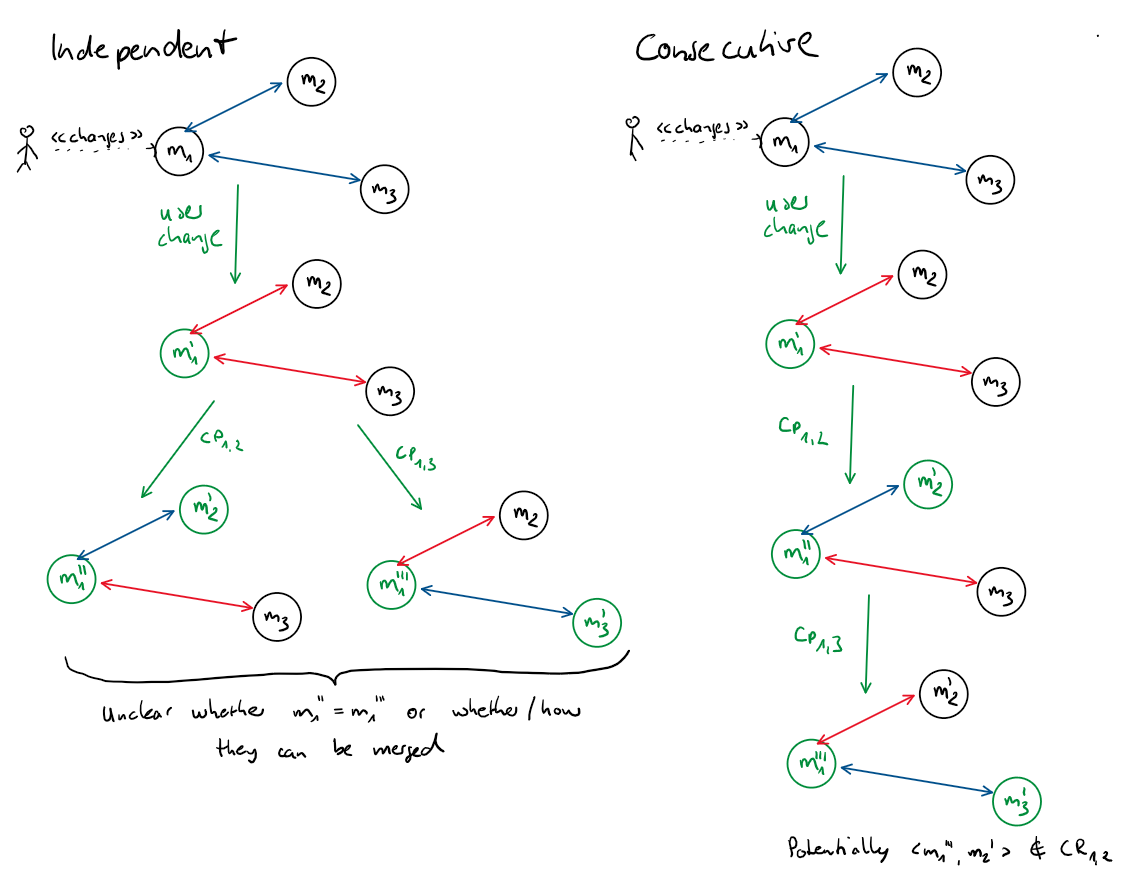
\includegraphics[width=\textwidth]{figures/correctness/notion/concurrent_consecutive_execution.png}
    \caption[Execution alternatives of consistency preservation rules]{Scenarios for independently executing consistency preservation rules on input models and consecutively executing them on the results of other rules.}
    \label{fig:correctness:concurrent_consecutive_execution}
\end{figure}

\mnote{Modular consistency preservation}
Like for the proposed notion of consistency, we can also consider consistency preservation in an either monolithic or modular way.
With a modular notion of consistency preservation, we may have multiple consistency preservation rules that preserve consistency, each of them for a consistency relation that defines consistency for a subset of the involved models.
Unlike for the relations defining consistency, which can be evaluated independently to identify whether models are consistent, the functions, i.e., consistency preservation rules, cannot be evaluated independently.
If each function is executed independently, they return new models that may need to be merged. 
This is exemplified in the following scenario, which is also depicted in \autoref{fig:correctness:concurrent_consecutive_execution}.
Imagine two functions $\function{Cp}_{1,2}$ and $\function{Cp}_{2,3}$ that preserve consistency for relations $\consistencyrelation{CR}{1,2}$ and $\consistencyrelation{CR}{2,3}$, respectively.
Consider the input models $\tupled{\model{m}{1}, \model{m}{2}, \model{m}{3}}$ that are not consistent to $\consistencyrelation{CR}{1,2}$ and $\consistencyrelation{CR}{2,3}$.
Now if we apply the functions independently, we have $\function{Cp}_{1,2}(\tupled{\model{m}{1}, \model{m}{2}}) = \tupled{\model{m}{1}', \model{m}{2}'} \in \consistencyrelation{CR}{1,2}$ and 
$\function{Cp}_{2,3}(\tupled{\model{m}{2}, \model{m}{3}}) = \tupled{\model{m}{2}'', \model{m}{3}''} \in \consistencyrelation{CR}{2,3}$.
It is now unclear how to unify $\model{m}{2}'$ and $\model{m}{2}''$ to $\model{m}{2}'''$, such that $\tupled{\model{m}{1}', \model{m}{2}'''} \in \consistencyrelation{CR}{1,2}$ and  $\tupled{\model{m}{2}''', \model{m}{3}''} \in \consistencyrelation{CR}{2,3}$.

\mnote{Consecutive function execution}
An intuitive approach to execute the functions is their composition, i.e., a consecutive execution that does not take the original models as input but the ones delivered by the previous executions of the functions for consistency preservation, which is also exemplarily depicted in \autoref{fig:correctness:concurrent_consecutive_execution}.
If we consecutively apply the two given functions, we know that $\function{Cp}_{1,2}(\tupled{\model{m}{1}, \model{m}{2}}) = \tupled{\model{m}{1}', \model{m}{2}'} \in \consistencyrelation{CR}{1,2}$ and 
$\function{Cp}_{2,3}(\tupled{\model{m}{2}', \model{m}{3}}) = \tupled{\model{m}{2}'', \model{m}{3}''} \in \consistencyrelation{CR}{2,3}$.
It is, however, unclear whether $\tupled{\model{m}{1}', \model{m}{2}''} \in \consistencyrelation{CR}{1,2}$, so it may be necessary to execute $\function{Cp}_{1,2}$ again.
In fact, we need some method to decide in which order and how often the consistency preservation rules are applied to result in a consistent tuple of models.
We call this an \emph{orchestration}.

\mnote{Unification or orchestration necessary}
%The examples for the two strategies of executing consistency preservation rules are depicted in \autoref{fig:correctness:concurrent_consecutive_execution}. 
Even if consistency preservation rules were supposed to only modify one model instead of two, the same problems of unifying changes of their independent execution or orchestration of their consecutive execution occur as soon as there are two sequences of consistency preservation rules that change the same models.

\mnote{Benefits of consecutive execution}
In our work, we follow the approach of orchestrating and consecutively executing consistency preservation rules.
The benefits of this approach are twofold. First, there is no additional logic required for unifying the changes performed by independently executed consistency preservation rules. 
Second, the unification may deliver a model that is not consistent to any of the consistency relations anymore, whereas consecutive execution at least gives the guarantee that the models are consistent to the last applied consistency preservation rule.
With this approach, the repeated execution of consistency preservation rules can be seen as a negotiation of a solution by reacting to the changes the others performed.

\begin{remark} 
\mnote{Monolithic notions as degraded modular ones}
Finally, every monolithic notion of consistency and its preservation can be considered a special case of a modular notion. Having only one consistency relation and one function that preserves it degrades the problem by making the necessity to perform an orchestration of functions obsolete.
\end{remark}

\mnote{Realization options for consistency preservation rules}
For now, the introduced consistency preservation rules can be any kind of functions that return consistent models. 
Their realization may, for example, be transformations that define how to react to certain changes for restoring consistency, or constraint solvers that find consistent models by solving consistency constraints. 
We do not yet need to consider how these functions are realized to derive consistent models, although, later, we will focus on transformation-based approaches.


\subsection{Declarative and Imperative Specifications}
\label{chap:correctness:notions_consistency:declarative_imperative}

\begin{figure}
    \centering
    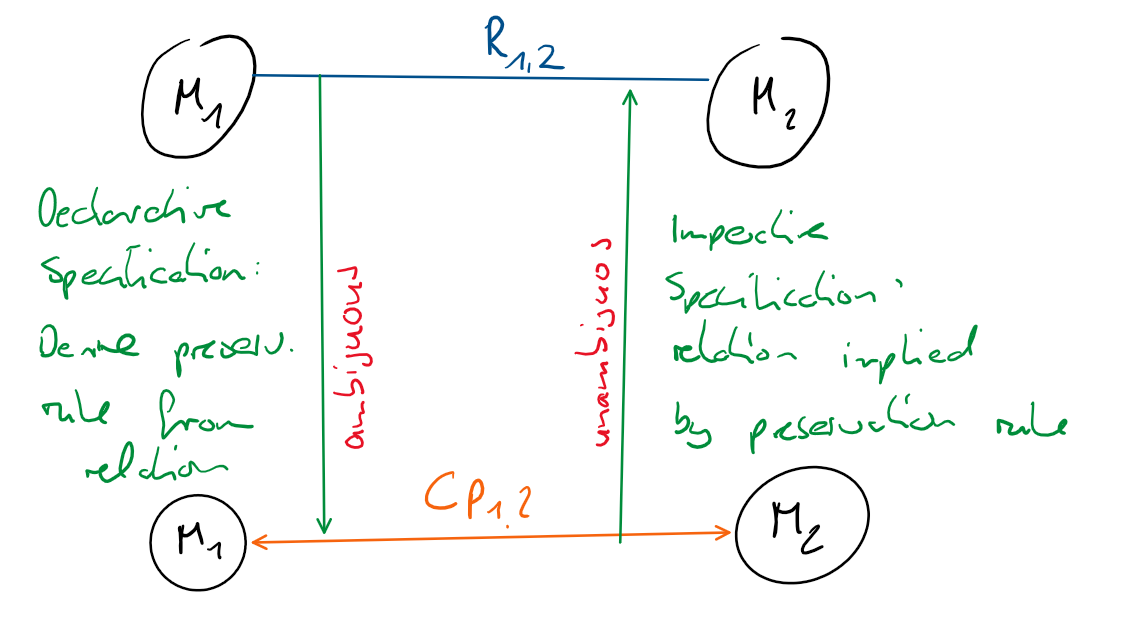
\includegraphics[width=0.5\textwidth]{figures/correctness/notion/declarative_imperative}
    \caption[Declarative and imperative consistency specification]{Declarative and imperative specification of consistency relations and consistency preservation rules for two metamodel $\metamodel{M}{1}$ and $\metamodel{M}{2}$.}
    \label{fig:correctness:declarative_imperative}
\end{figure}

\mnote{Only define relation or function}
We have discussed that consistency preservation can be considered as functions, called consistency preservation rules, that preserve consistency according to some relations.
%In practice, consistency preservation is usually specified by means of transformations.
In practice, however, one will usually not specify both the consistency relation itself and also the consistency preservation rule that preserves it.
Instead, usually one artifact is given and the other is implied or derived.
This leads to the two approaches of \emph{declarative} and \emph{imperative} consistency specifications, depending on whether the specification defines \emph{how} consistency is achieved.
The relation between the two approaches and a consistency relation as well as a consistency preservation rule is depicted in \autoref{fig:correctness:declarative_imperative}.

\mnote{Ambiguity in deriving rules}
As a first option, a developer may only define relations that specify consistency. Functions that preserve these relations can be derived from that.
This is called a \emph{declarative} specification, because it only declares when models are consistent but not \emph{how} consistency is achieved.
In general, there is not only a single option how this function can look like.
It can, for example, calculate the result with minimal differences to the input, according to some defined metrics.
Or, especially if there is an intensional specification of the relations, the approach may consider the type of input change and calculate an appropriate change according to the constraints in the intensional specification.
This approach is followed by many declarative transformation languages, such as \gls{QVTR}~\cite{qvt}, or \glspl{TGG}~\cite{anjorin2014EfficientSynchronizationTGG-ECMFA}.

\mnote{Relations as fixed points}
As a second option, a developer can define consistency preservation rules without explicitly specifying the consistency relations to which they preserve consistency.
Instead, these functions imply the underlying consistency relations that they preserve, at least if we assume that a consistency preservation rule does not perform changes when the input models are already consistent.
% If a consistency preservation rule $\function{Cp}$ ensures that its application returns a consistent model, the consistency relation $\consistencyrelation{CR}{}$ it preserves is given by its image: 
% $\consistencyrelation{CR}{} = \setted{\modeltuple{m} \mid \exists \modeltuple{m}' : \function{Cp}(\modeltuple{m}') = \modeltuple{m}}$.
% If a consistency preservation rule at least ensures that the models are consistent if its application does not perform any changes, the consistency relation $\consistencyrelation{CR}{}$ it preserves is given by its fixed points:
% $\consistencyrelation{CR}{} = \setted{\modeltuple{m} \mid \function{Cp}(\modeltuple{m}) = \modeltuple{m}}$.
Given a function $\function{Cp}$, the relation $\consistencyrelation{CR}{}$ it preserves is implied by its fixed points: $\consistencyrelation{CR}{} = \setted{\modeltuple{m} \mid \function{Cp}(\modeltuple{m}) = \modeltuple{m}}$.
If a function preserving consistency does not perform any changes, the models are, by definition, consistent.
Usually, we will assume that such a function returns consistent models with a single application.
Thus, if it does not perform changes when the input models are already consistent, the function is idempotent and then the consistency relation is given by its image, i.e., $\consistencyrelation{CR}{} = \setted{\modeltuple{m} \mid \exists \modeltuple{m}' : \function{Cp}(\modeltuple{m}') = \modeltuple{m}}$.
This is called an \emph{imperative} specification, because it declares \emph{how} consistency can be achieved.
Such an approach is followed by many imperative transformation languages, such as \gls{QVTO}~\cite{qvt}. % or \gls{VIATRA}.


\subsection{Consistency Preservation Artifacts}

\mnote{Four artifacts}
We have discussed that consistency can be considered in a monolithic or modular way. We have, however, also mentioned that the monolithic case can be considered as a special case of the modular one.
For the general case, we thus know from the previous considerations that in a consistency preservation process at least specifications that define consistency, called \emph{consistency relations}, functions that preserve consistency, called \emph{consistency preservation rules}, and a function for orchestrating the functions, in the following called \emph{orchestration function}, are necessary. Finally, we also need a function that applies the consistency preservation rules in the order that is determined by the orchestration function, which we call the \emph{application function}.
To summarize, we consider the following artifacts necessary to handle consistency preservation:
\begin{properdescription}
    \item[Consistency Relations:] Binary relations that specify when models are to be considered consistent.
    \item[Consistency Preservation Rules:] Functions that restore consistency for a pair of models that became inconsistent by modification.
    \item[Orchestration Function:] A function that determines the execution order of the consistency preservation rules to restore consistency.
    \item[Application Function:] A function that applies the consistency preservation rules in the order determined by the orchestration function. 
\end{properdescription}

\begin{figure}
    \centering
    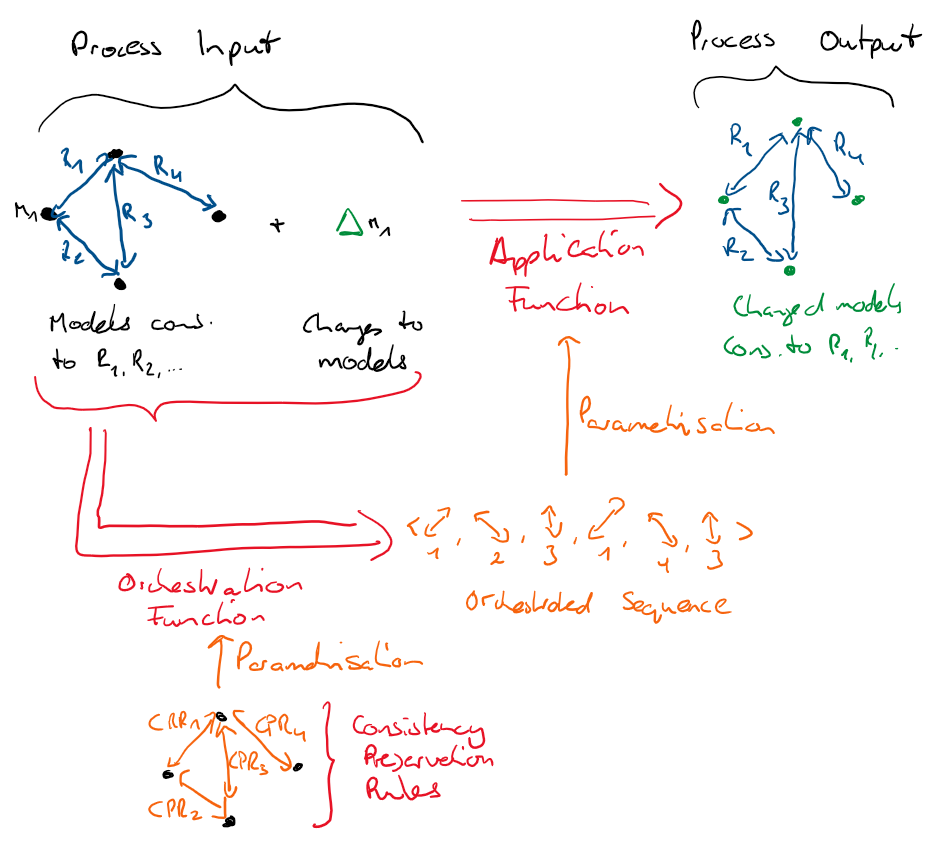
\includegraphics[width=\textwidth]{figures/correctness/notion/execution_process.png}
    \caption[Consistency specification execution process and artifacts]{Execution process and artifacts for a modular consistency specification. Relevant artifacts are annotated in red, changes generated by the process are depicted in green, parametrizations of the functions are depicted in orange.}
    \label{fig:correctness:execution_process}
\end{figure}

\mnote{Distinction between orchestration and application}
We explicitly distinguish the orchestration and the application to be able to make more fine-grained statements about the responsibilities for the orchestration and its actual execution, especially to determine the behavior in cases when no orchestration is found in which the transformations can be applied to yield consistent models.
The process is depicted in \autoref{fig:correctness:execution_process}. Given models that are consistent according to some consistency relations and changes to them that lead to inconsistencies, the orchestration function delivers an order of consistency preservation rules, which is used to parametrize the application function that executes these rules in the given order.
The result is, in the best case, a model tuple that is consistent to the relations again.
%However, we will see that this is not always possible. %Thus, we will especially discuss relevant properties of the artifacts, such as correctness and optimality that reflect how and when this process can be executed successfully.

